\documentclass[french]{beamer}

\usepackage[utf8]{inputenc}
\usepackage[T1]{fontenc}
\usepackage{lmodern}
\usepackage{amsmath, amssymb}

\usepackage{babel}

%CHOIX DU THEME et/ou DE SA COULEUR
%\usetheme{PaloAlto}
%\usetheme{Madrid}

\usetheme{Copenhagen}

% => il est possible, pour un thème donné, de modifier seulement la couleur
%\usecolortheme{crane}
\usecolortheme{seahorse}
%\useoutertheme[left]{sidebar}

\title{Projet collaboratif : Pollen}
\subtitle{Partie Élasticité linéaire}
\author{Nabil Belahrach \& Alexandre Corizzi}
\date{Novembre 2015}
\institute{Université de Strasbourg -- U.F.R. de Mathèmatiques
et d'Informatique}

\begin{document}
\newcommand*\diff{\mathop{\!\mathrm{d}}}
\AtBeginSection[{\begin{frame}{Outline}
    \tableofcontents[hideothersubsections, pausesections] 
\end{frame}}]

\addtobeamertemplate{footline}{\insertframenumber/\inserttotalframenumber}

\begin{frame}
  \titlepage
\end{frame}
\begin{frame}{Plan}
  \tableofcontents
\end{frame}

% ------------------------------------------------------------------------------
\section{Présentation du problème}
\begin{frame}
  \vfill
  \centering
  \begin{beamercolorbox}[sep=8pt,center,shadow=true,rounded=true]{title}
    \usebeamerfont{title}\insertsectionhead
  \end{beamercolorbox}
  \vfill
\end{frame}
% ------------------------------------------------------------------------------

\begin{frame}{Schéma de la buse}
  \begin{center}
    \begin{figure}
      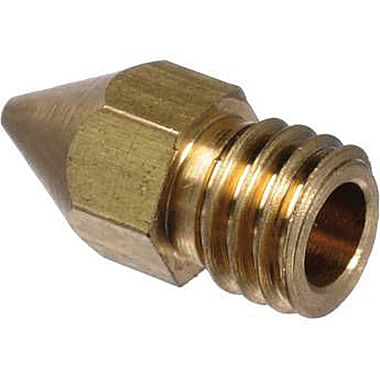
\includegraphics[scale=0.3]{images/buse.png}
      \caption{Buse reliée à la vis d'extrusion}
    \end{figure}
  \end{center}
\end{frame}

\begin{frame}{Schéma de la buse}
  \begin{minipage}{0.48\textwidth}
    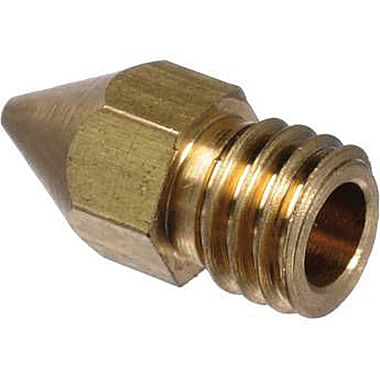
\includegraphics[scale=0.3]{images/buse.png}
  \end{minipage}
  \hspace*{\stretch{1}}
  \begin{minipage}{0.48\textwidth}
    Propriétés élastiques :
    \begin{itemize}
      \item Matériau homogéne isotrope
	\pause
      \item Loi de Hooke en 3D  
    \end{itemize}
  \end{minipage}
\end{frame}


\begin{frame}{Schéma de la buse}
  \begin{minipage}{0.48\textwidth}
    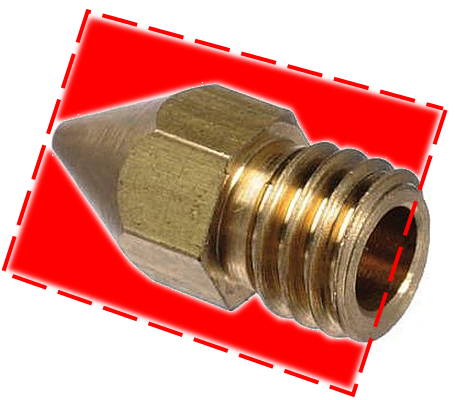
\includegraphics[scale=0.3]{images/buseCoupe.png}
  \end{minipage}
  \hspace*{\stretch{1}}
  \begin{minipage}{0.48\textwidth}
    Propriétés géométriques :
    \begin{itemize}
      \item Axisymétrique
	\pause
      \item Utilisation de Coordonnées cylindriques
	\pause
      \item Passage à un Problème 2D
    \end{itemize}
  \end{minipage}
\end{frame}

% ------------------------------------------------------------------------------

\section{Formulation des équations}
\begin{frame}
  \vfill
  \centering
  \begin{beamercolorbox}[sep=8pt,center,shadow=true,rounded=true]{title}
    \usebeamerfont{title}\insertsectionhead
  \end{beamercolorbox}
  \vfill
\end{frame}
% ------------------------------------------------------------------------------

\subsection{Principaux acteurs}
\begin{frame}{Déplacement et déformation}
  \begin{itemize}
    \item Vecteurs de deplacement (inconnus) : $\vec{u} \in \mathbb{R}^3 $
  \end{itemize}
  \pause
  \vspace{2pt}

  \begin{equation}
    \nabla u =  
    \left(
    \begin{array}{ccc}
      \frac{\partial u_x}{\partial x } & \frac{\partial u_x}{\partial y } & 
      \frac{\partial u_x}{\partial z }  \\
      \frac{\partial u_y}{\partial x } & \frac{\partial u_y}{\partial y } & 
      \frac{\partial u_y}{\partial z }  \\
      \frac{\partial u_z}{\partial x } & \frac{\partial u_z}{\partial y } & 
      \frac{\partial u_z}{\partial z } 
    \end{array}
    \right)
  \end{equation}
  \pause
  \vspace{2pt}
  \begin{itemize}
    \item On définit le \emph{tenseur des déformations} symétrique : 
  \end{itemize}

  \begin{equation}
    \boxed{\varepsilon = \frac{1}{2} \left( \nabla u + ^{t} \nabla u \right)} 
    \in \mathcal{M}_{3,3}(\mathbb{R})
  \end{equation}

\end{frame}


\begin{frame}{Loi de Hooke}

   \emph{Relation linéaire entre une force et une déformation.}
   \pause
  \begin{equation}
    \sigma \left(\vec{u}\right) = \left( \lambda \hspace{2pt}\mathbf{div} 
    \hspace{2pt}\vec{u} \cdot \mathbf{I} \right) + 2 \mu\cdot \varepsilon 
  \end{equation}
  \begin{itemize}
      \pause
    \item $\lambda$ et $\mu$ sont les coéffiscients de Lamé du matériau. \\
      \pause
      $\mu$ est la résistance au cisaillement 
      \pause
     \item $\sigma \in \mathcal{M}_{3,3}(\mathbb{R})$ : tenseur des contraintes (efforts intérieurs)
    
  \end{itemize}
\end{frame}


\subsection{Problème aux Valeurs Propres} 
\begin{frame}{Problème aux Valeurs Propres} 
  \begin{equation*}
    - \mathbf{div}  \left( \sigma \left(\vec{u}\right) \right) = \vec{\mathbf{F}}_{ext}
  \end{equation*}

  \begin{equation}
   - \mathbf{div}  \left( \sigma \left(\vec{u}\right) \right) = \lambda \cdot \vec{u}
  \end{equation}
\end{frame}

\subsection{Formulation faible}
\begin{frame}
  \begin{equation}
    - \int_\Omega \mathbf{div}  \left( \sigma \left(u\right) \right) v \hspace{7pt} \diff \Omega 
    = \int_\Omega \lambda \hspace{2pt} u v \hspace{7pt} \diff \Omega
  \end{equation}
  \pause
  On a d'abord :
  \begin{equation*}
    \left[\mathbf{div}  \left( \sigma \left(\vec{u}\right) \right)\right]_i = 
    \sum_{j=1}^3 \frac{\partial\sigma_{i,j}}{\partial x_j}, \hspace{28pt}  \boxed{1 \leq i \leq 3}
      \end{equation*}
  \pause
  \vspace{10pt}
  Et donc : 
  \begin{equation}
    ^{\mathrm{GREEN}}\Leftrightarrow
      \int_\Omega \sum_{j=1}^3 \sigma_{i,j} \frac{\partial v_i}{\partial x_j} \diff \Omega 
      \underbrace{- \int_\Gamma \sum_{j=1}^3 \left(\sigma_{i,j}, \vec{\mathbf{n}} \right) v_i \hspace{7pt} 
       \diff \Gamma}_{\mathrm{BC}}
    = \int_\Omega \lambda_i \hspace{2pt} u_i v_i \hspace{7pt} \diff \Omega
  \end{equation}
  \end{frame}


\subsection{Changement de variables} 
\begin{frame}{Coordonnées cylindriques}
  \begin{minipage}{0.48\textwidth}
    \begin{equation*}
      \left \{
	\begin{array}{ccc}
	  x & = &r \cos \theta  \\
	  y & = &r \sin \theta   \\
	  z & = &z \\
	\end{array}
	\right.
      \end{equation*}
    \end{minipage}
    \hspace*{\stretch{1}}
    \begin{minipage}{0.48\textwidth}
      \begin{equation}
	\left \{
	  \begin{array}{ccc}
	    u_x & = &u_r \cos \theta  \\
	    u_y & = &u_r \sin \theta   \\
	    u_z & = &u_z \\
	  \end{array}
	  \right.
	\end{equation}
      \end{minipage}
      \pause
    \vspace{23pt}
  \begin{equation}
    J  =  
    \left(
    \begin{array}{ccc}
         \cos \theta &  \sin \theta & 0 \\
      -r \sin \theta &r \cos \theta & 0 \\
                          0 & 0 & 1 \\
    \end{array}
    \right)
  \end{equation}
\end{frame}

\begin{frame}{Transformation inverse pour le changement de variable}
\begin{equation}
    \left \{
      \begin{array}{rcl}
	\frac{\partial g}{\partial x} & = & \frac{\partial g}{\partial r} 
	\cos \theta - \frac{1}{r} \frac{\partial{g}}{\partial \theta} \sin \theta 
	\vspace{10pt} \\
	\frac{\partial g}{\partial y} & = & \frac{\partial g}{\partial r} 
	\sin \theta + \frac{1}{r} \frac{\partial{g}}{\partial \theta} \cos \theta
	\vspace{10pt} \\
	\frac{\partial g}{\partial z} & = & \frac{\partial g}{\partial z}\\
      \end{array}
      \right.
    \end{equation}
\end{frame}

% ------------------------------------------------------------------------------
  \section{Éxpérimentation}
  \begin{frame}
    \vfill
    \centering
    \begin{beamercolorbox}[sep=8pt,center,shadow=true,rounded=true]{title}
      \usebeamerfont{title}\insertsectionhead
    \end{beamercolorbox}
    \vfill
  \end{frame}
% ------------------------------------------------------------------------------

  \begin{frame}{Code FreeFem++}
  \end{frame}

  \end{document}

